\documentclass[12pt,twoside]{article}
\usepackage[dvipsnames]{xcolor}
\usepackage{tikz,graphicx,amsmath,amsfonts,amscd,amssymb,bm,cite,epsfig,epsf,url}
\usepackage[hang,flushmargin]{footmisc}
\usepackage[colorlinks=true,urlcolor=blue,citecolor=blue]{hyperref}
\usepackage{amsthm,multirow,wasysym,appendix}
\usepackage{array,subcaption} 
% \usepackage[small,bf]{caption}
\usepackage{bbm}
\usepackage{pgfplots}
\usetikzlibrary{spy}
\usepgfplotslibrary{external}
\usepgfplotslibrary{fillbetween}
\usetikzlibrary{arrows,automata}
\usepackage{thmtools}
\usepackage{blkarray} 
\usepackage{textcomp}
\usepackage[left=0.8in,right=1.0in,top=1.0in,bottom=1.0in]{geometry}
\newcommand{\rnd}{\Tilde}
\newcommand{\ru}{\rnd{ u}  }
\newcommand{\rd}{\rnd{ d}  }
%\newcommand{\rs}{\rnd{ s}  }
\newcommand{\ri}{\rnd{ i}  }
\newcommand{\re}{\rnd{ e}  }
\newcommand{\rQ}{\rnd{ q}  }
\newcommand{\rC}{\rnd{ c}  }
\newcommand{\rb}{\rnd{ b}  }
\newcommand{\ra}{\rnd{ a}  }
\newcommand{\E}{E}
\newcommand{\R}{\mathbf{R}}
\newcommand{\brac}{}
\newcommand{\cnd}{|}
\newcommand{\Var}{Var}
\usepackage{pdfpages}

\title{Hw7}
\author{gjd9961 }
\date{November 2021}

\begin{document}

\maketitle

\begin{enumerate}


\item (Short questions) 
Justify all your answers mathematically.
\begin{enumerate}
\item For any random variable $\ra$, can  $\E^2(\ra)$ be smaller than $\E(\ra^2)$?  
\subitem
Yes, this can be true. We know that 
$$
    E(\ra^2) - \E^2(\ra)= E((\ra - E(\ra))^2) 
$$
Which can be expressed as 
$$
    E((\ra - E(\ra))^2) = \sum_{a\in \R_{\ra}} p(_\ra(a)) \times (a-E(\ra))^2 
$$
And since probabilities are non negative by definition, and the other term is being squared, we have two positive quantities multiplying each other and then getting summed. Therefore, we cannot have a negative value for $E((\ra - E(\ra))^2)$ which means that $E((\ra - E(\ra))^2) \geq 0$ and $\E(\ra^2) - \E^2(\ra) \geq 0$ and that $E^2(\ra) \leq E(\ra^2)$
\item If $\ra$ and $\rb$ have the same distribution and are independent, is it true that $\E(\ra \rb) = \E^2(\ra)$?
\subitem Yes this is true, and we can leverage the fact that they are independent and that if they have the same distribution they have the same expectation ($E(\ra) = E(\rb)$) to show that $\E(\ra \rb) = \E^2(\ra)$:
$$
    E(\ra \times \rb) = E(\ra) \times E(\rb) = E(\ra) \times E(\ra) = E^2(\ra) \qed
$$
\item A teacher of a class of $n$ children asks their parents to leave a present under the Christmas tree in the classroom. The day after, each child picks a present at random. What is the expected number of children that end up getting the present bought by their own parents? (Hint: Define a random variable $I_i$ that is equal to one when kid $i$ gets the present bought by their own parents, and to zero otherwise.)
\subitem
Since there are $n$ kids in the classroom, there will be $n$ presents under the tree. Picking at random, any child will have a $\frac{1}{n}$ chance of getting the present their parents left. Well define the present a child pics as a random variable $\ri$ and when $\ri=0$ then the child did not get the present their parent left, and when $\ri = 1$ then they did.
$$
    P_{\ri}(\ri=0) = 1-\frac{1}{n} \text{   and   } P_{\ri}(\ri = 1) = \frac{1}{n}
$$
Since there are n kids and $P_{\ri}(\ri=1)=\frac{1}{n}$ then the expectation is calculated as follows:
$$
    E(\text{Kids that get their parents present}) = E(\sum_{i=1}^n E(\ri)) = n \times \frac{1}{n} = 1
$$

That means that on average, one child in the classroom should get the present their parents left under the tree by random chance alone. 

\end{enumerate}


\item (Computer) We model the time (in years) until a computer breaks down as a random variable $\rnd{t}$. The time depends on whether the computer has a defect or not, which is modeled by a random variable $\rnd{d}$. If the computer has a defect ($\rnd{d}=1$), then $\rnd{t}$ is an exponential with parameter 2. If it does not ($\rnd{d}=0$), then $\rnd{t}$ is an exponential with parameter 1. The probability that the computer has a defect is 0.1.
\begin{enumerate}
\item Is the conditional expectation of $\rnd{t}$ given $\rnd{d}$ a discrete or continuous random variable? What is its pmf or pdf? 
\subitem 
Since we're plugging a random variable into a continuos function, our conditional expectation of  $\rnd{t}$ given $\rnd{d}$ is a continuos random variable. Its pdf can be described in the following way:
$$
PDF = f_{t|d}(t|d) = 
    \begin{cases}
    Exp(2) & \text{ if } \rnd{d}=1 \\
    Exp(1) & \text{ if } \rnd{d}=0
    \end{cases}
$$
\item What is the variance of $\rnd{t}$?
\subitem
If we want to compute the variance of $\rnd{t}$ we must first compute the marginal
$$
    Marignal = \sum_0^1 P_d{d}f_{t|d}(t|d) = p_d(0)f_{t|0}(t|0) + p_d(1)f_{t|1}(t|1) = .9 \times e^{-t} + .1\times e^{-2t}
$$
Now we can continue to compute the expectation for $\rnd{t}$ and $\rnd{t^2}$ and then the variance
$$
    E(t) = \int_0^\infty \rnd{t}f_t(t) = 0.95 \text{ and } E(t^2) = \int_0^\infty \rnd{t^2}f_t(t) = 1.85
$$
Finally:
$$
    Var(\rnd{t}) = E(t^2)-E(t)^2 = 1.85 - .95^2 = .0.9475
$$
\item A company buys 100 of these computers. If the time until they break down is distributed as explained above, and they are all independent, what is the mean and variance of the number of computers that break down during the first year?
\subitem 
We could model the nubmer of computers that breaks down during the first year by modeling the 100 computers in a binomial distribution. Our size would be 100, and our probability would be .65 as
$$
    f_{t|t,d}(t|t,d) = \int_0^1 f_{t}(t) = .65
$$
Thus the mean of the distribution would be $n\times p = 65$ and the \textbf{Variance} would be $n\times p(1-p) = 100 \times .65 \times (1-.65) = 22.75 $
\end{enumerate}

\item (Law of conditional variance) 
In this problem we define the conditional variance in a similar way to the conditional expectation. 
\begin{enumerate}
\item What is the object $\Var ( \rb \cnd \ra = a)$ (i.e. is it a number, a random variable or a function)? What does it represent?
\subitem At the end of the day, it just represents a number, the variance of a random variable $\rb$ given some information about the random variable $\ra$. This is because once we observe a value of $\ra$, $a$ becomes fixed, and then when we look at joint density of the two random variables and then condition on the event $a$ we observed, we get a new distribution. Then the variance of the distribution is a fixed number, the mathematical object in question.
\item Setting $h(a) = \Var (\rb \cnd \ra = a)$ we define the conditional variance as $\Var (\rb \cnd \ra) = h(\ra)$. What is this object? 
\subitem
Now what we have is not a number, because $\ra$ is not observed and fixed to any given number, that is to say, we're not sure exactly what to condition on. We know that if we define a function in terms of random variables, the resulting function is a random variable, thus, the object we have on our hands is a random variable. 
\item Prove the law of conditional variance:
\begin{align}
\Var (\rb) = \E ( \Var(\rb \cnd \ra) ) + \Var ( \E (\rb \cnd \ra))
\end{align}
and describe it in words.
\subitem
We can prove this in the following way:
\begin{equation}
    \begin{split}
        E(\Var (\rb|\ra)) &= \E (\E(\rb^2 \cnd \ra) ) - \E ( \E (\rb \cnd \ra)^2))\\
        E(\Var (\rb|\ra)) &= \E(\rb^2) - \E ( \E (\rb \cnd \ra)^2) \\
        &\text{ and } \\ 
        Var(E(\rb|\ra)) &= E(E(\rb|\ra)^2) - E(E(\rb|ra))^2 \\\
        Var(E(\rb|\ra)) &= E(E(\rb|\ra)^2) - E(\rb)^2 
    \end{split}
\end{equation}
Using what we computed, we can substitute these identities in and what we now have is: 
\begin{equation}
    \begin{split}
        E(Var(\rb|\ra) + Var(E(\rb|\ra)) &= E(\rb^2) - E(\rb)^2 \\
        E(\rb^2) - E(\rb)^2 &= Var(\rb)
    \end{split}
\end{equation}
What we have shown is that the Expectation of the variance of a random variable given some information about another random variable plus the variance of the expectation of a random variable given some information about a random variable is equal to the variance of the primary random variable (not the one being conditioned on). 
%\item We model the time at which a runner gets injured (in hours) during a marathon as an exponential random variable with parameter equal to 1 if the runner is under 30 years old and 2 if she is over 30. What is the mean and the standard deviation of the time at which a runner gets injured if $20 \%$ of the runners are over 30?
\end{enumerate}

\item (Water salinity and temperature)  %A quick Google search will tell you that the salinity of water, which is the salt content in water, increases with temperature. This is because water expands at larger temperature and can fit in more molecules, including salt, increasing the salinity (according to \href{https://sciencing.com/salinity-impact-oceans-currents-5517246.html}{Sciencing}). 
In this question, we use \href{https://www.kaggle.com/sohier/calcofi}{oceanographic data } to study the relationship between salinity and temperature in sea water. We perform our analysis on a cleaned and subsampled version of the data, \texttt{bottle.csv}.  %Please refer to the Kaggle website for any details about the data. 
The script is available at \url{https://github.com/cfgranda/prob_stats_for_data_science/blob/main/hw7/conditional_expectation_EXERCISE.ipynb}
\begin{enumerate}
%\item  Find the best linear MMSE estimator of salinity with temperature . Plot the line and the scatter plot of data on the same graph. According to the relationship you uncovered here, does water salinity increase with temperature? 
\item Plot an estimate of the conditional mean of salinity given the temperature along with the scatter plot of data. Justify any choices you make. %(Hint: this question closely follows example 5.2)
\item Annotate your plot to incorporate the conditional standard deviation of salinity given the temperature (apart from plotting the conditional mean, plot the conditional mean $\pm$ the conditional standard deviation).
\item Do you expect your estimates to be equally reliable at every point? Please explain your reasoning. (We are not looking for a mathematical answer, you can just explain intuitively.)

No, they definitely wont be reliable at every point. There were choices made about bucketing the data, and  some buckets (such as from $0 < t < 6$ or even $25 < t < 30$) that might have less values than the others and therefore their means will be less reliable compared to other buckets containing more values (such as $10 < t < 20$). 

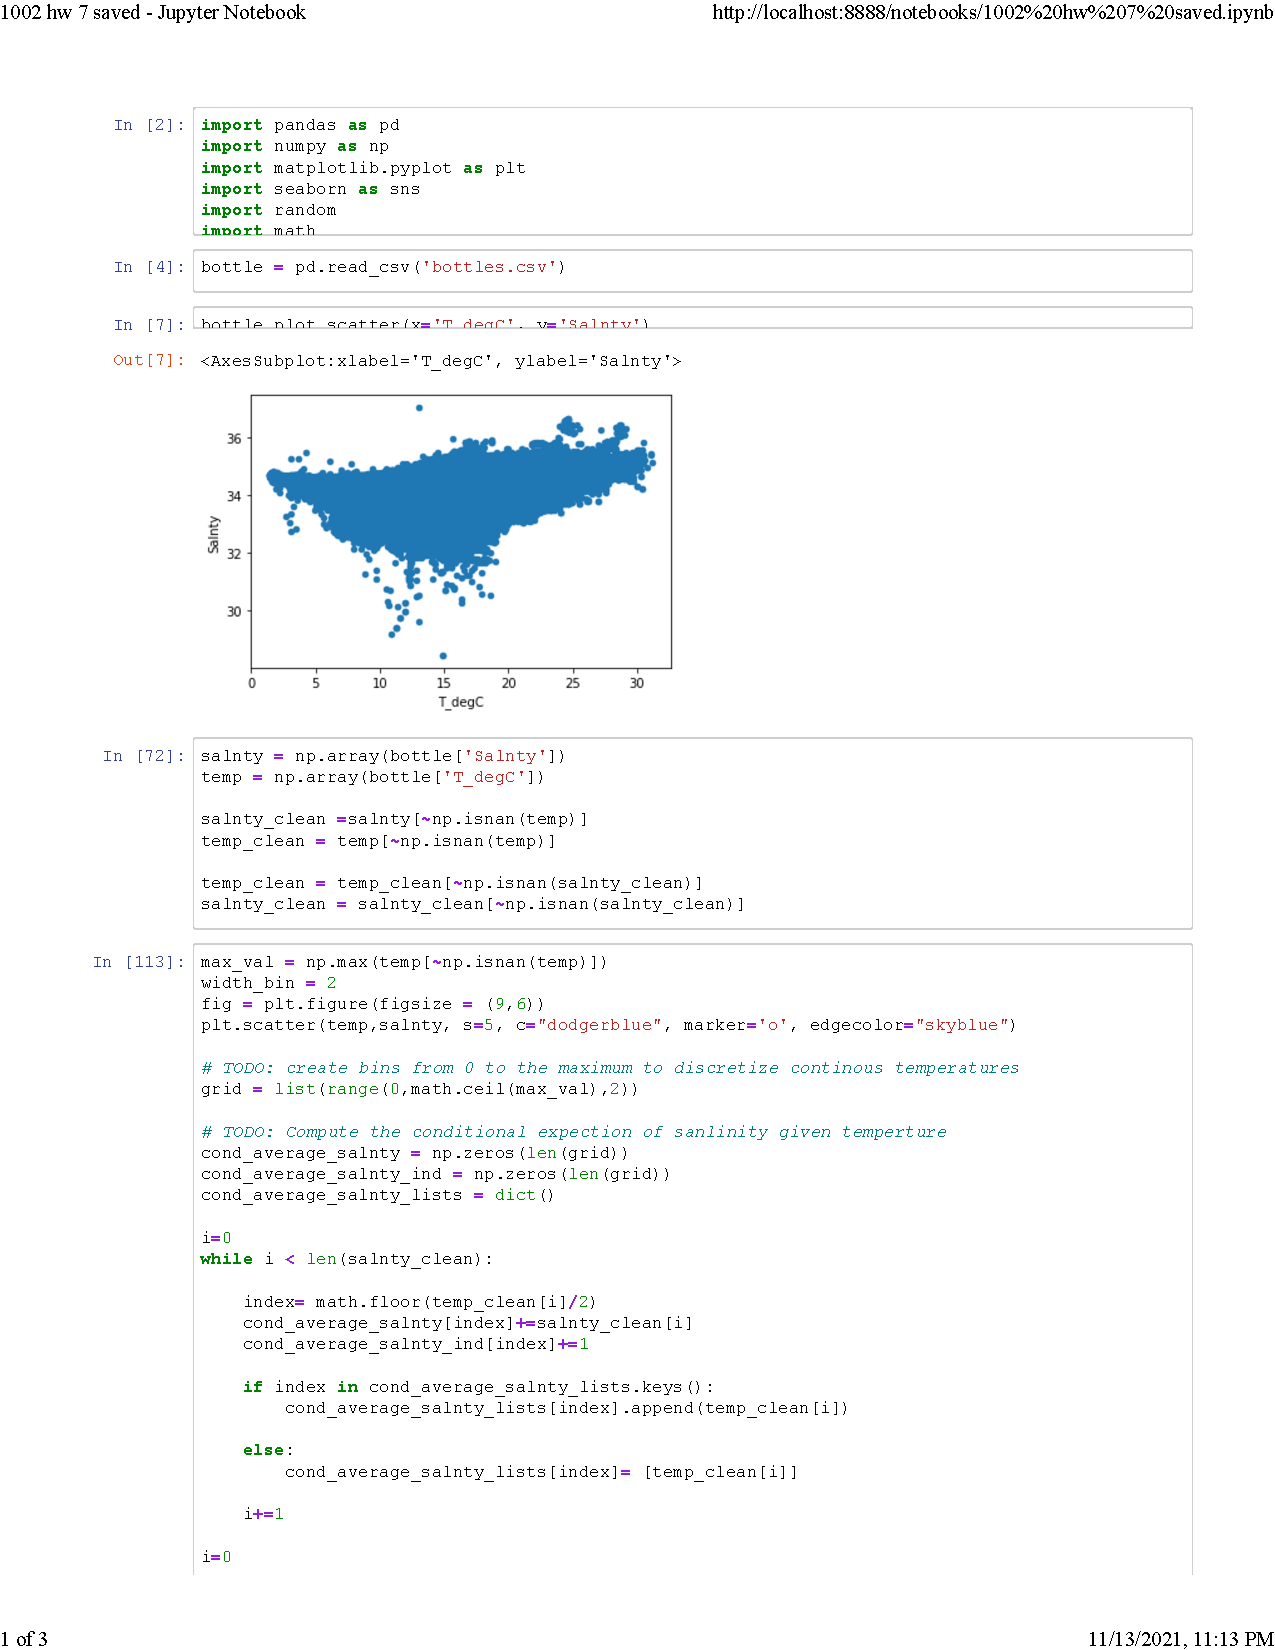
\includepdf[pages=-]{1002hw7jupy.pdf}
%\item (Not graded for points) Why do you think the trend you find is different from what  \href{https://sciencing.com/salinity-impact-oceans-currents-5517246.html}{Sciencing} suggests? It is not because of limited data - the full dataset has $810k$ data points and we still observe the same trend. 

\end{enumerate}


\end{enumerate}
\end{document}
